

\section{GMRES Iteration}
\label{sec:3}

\subsection{The minimization property and its consequences}
\label{sec:3.1}

\begin{thm}[The minimization property of GMRES iteration]
  Let $A$ be nonsingular. The $k$th iteration of GMRES is the solution
  to the least squares
  problem
  \begin{equation}
    \label{eq:3.1}
    \text{minimize}_{x\in x_0+\mathcal{K}_k}\|b-Ax\|_2.
  \end{equation}
  Then for all $\overline{p}_k\in\mathcal{P}_k$
  \begin{equation}
    \label{eq:3.2}
    \|r_k\|_2=\min_{p\in\mathcal{P}_k}\|p(A)r_0\|_2\leq \|\overline{p}_k(A)r_0\|_2
  \end{equation}
\end{thm}

\begin{proof}
  Note that if $x\in x_0+\mathcal{K}_k$,
  then $$x=x_0+\sum\limits_{j=0}^{k-1}\gamma_{j}A^jr_0$$
  and so
  $$b-Ax=b-Ax_0-\sum\limits_{j=0}^{k-1}\gamma_{j}A^{j+1}r_0
  =r_0-\sum\limits_{j=1}^{k}\gamma_{j-1}A^jr_0$$
  Hence if $x\in x_0+\mathcal{K}_k$ then $r=\overline{p}(A)r_0$ where
  $\overline{p}\in\mathcal{P}_k$ is a residual polynomial, so
  \eqref{eq:3.2} is proved.
\end{proof}

\begin{coro}
  Let $A$ be nonsingular and let $x_k$ be the $k$th GMRES
  iteration. Then for all $\overline{p}_k\in\mathcal{P}_k$
  \begin{equation}
    \label{eq:3.3}
    \frac{\|r_k\|_2}{\|r_0\|_2}\leq \|\overline{p}_k(A)\|_2.
  \end{equation}
\end{coro}

\begin{thm}
  Let $A$ be nonsingular. Then the GMRES algorithm will find the
  solution within $N$ iterations.
\end{thm}

\begin{proof}
  The characteristic polynomial of $A$ is $p(z)=\det(A-zI)$. $p$ has
  degree $N$ and $p(0)=\det(A)\neq 0$ since $A$ is nonsingular, so
  $$\overline{p}_N(z)=p(z)/p(0)\in\mathcal{P}_N$$
  is a residual polynomial. It is well known that
  $p(A)=0=\overline{p}_N(A).$ By \eqref{eq:3.3}, $r_N=b-Ax_N=0$ and
  hence $x_N$ is the solution.
\end{proof}

\begin{thm}
  Let $A=V\Lambda V^{-1}$ be a nonsingular diagonalizable matrix. Let
  $x_k$ be the $k$th GMRES iterate. Then for all
  $\overline{p}_k\in\mathcal{P}_k$
  \begin{equation}
    \label{eq:3.4}
    \frac{\|r_k\|_2}{\|r_0\|_2}\leq \kappa_2(V)\max_{z\in\sigma(A)}|\overline{p}_k(z)|.
  \end{equation}
\end{thm}

\begin{proof}
  Let $\overline{p}_k\in\mathcal{P}_k.$ We can easily estimate
  $\|\overline{p}_k(A)\|_2$ by
  $$\|\overline{p}_k(A)\|_2\leq
  \|V\|_2\|V^{-1}\|_2\|\overline{p}_k(\Lambda)\|_2\leq
  \kappa_2(V)\max_{z\in\sigma(A)}|\overline{p}_k(z)|,$$
  as asserted.
\end{proof}

\begin{coro}
  If $A$ is normal, then we have
  $$\frac{\|r_k\|_2}{\|r_0\|_2}\leq\max_{z\in\sigma(A)}|\overline{p}_k(z)|.$$
\end{coro}

\begin{thm}
  Let $A$ be a nonsingular diagonalizable matrix. Assume that $A$ has
  only $k$ distinct eigenvalues. Then GMRES will terminate in at most
  $k$ iterations.
\end{thm}

\begin{thm}
  Let $A$ be a nonsingular normal matrix. Let $b$ be a linear
  combination of $k$ of the eigenvectors of $A$
  $$b=\sum\limits_{l=1}^k\gamma_lu_{i_l}.$$
  Then the GMRES iteration, with $x_0=0,$ for $Ax=b$ will terminate in
  at most $k$ iterations.
\end{thm}

\subsection{Termination}
\label{sec:3.2}

\begin{exm}
  Assume that $A=V\Lambda V^{-1}$ is diagonalizable, that the
  eigenvalues of $A$ lie in the interval $(9,11)$, and that
  $\kappa_2(V)=100$. We assume that $x_0=0$ and hence $r_0=b$. Using
  residual polynomial $\overline{p}_k(z)=(10-z)^k/10^k$ we find
  $$\frac{\|r_k\|_2}{\|r_0\|_2}\leq (100)10^{-k}=10^{2-k}.$$
  Hence
  \begin{equation}
    \label{eq:3.5}
    \|r_k\|_2\leq\eta\|b\|_2
  \end{equation}
  holds when $k>2+\log_{10}(\eta).$
\end{exm}

\begin{lemma}
  Assume that $A$ is nonsingular, diagonalizable and $\|I-A\|_2\leq \rho<1.$ Let
  $\overline{p}_k(z)=(1-z)^k.$
  We have
  \begin{equation}
    \label{eq:3.6}
    \|r_k\|_2\leq \rho^k\|r_0\|_2.
  \end{equation}
\end{lemma}

\begin{rmk}
  The estimate \eqref{eq:3.6} illustrates the potential benefits of a
  good approximate inverse precondition.
\end{rmk}

\subsection{Preconditioning}
\label{sec:3.3}

\begin{defi}
  If one can find $M$ such that $$\|I-MA\|_2=\rho<1,$$
  then applying GMRES to $MAx=Mb$ allows one to apply \eqref{eq:3.6}
  to the preconditioned system. Preconditioning done in this way is
  called \emph{left preconditioning}.
\end{defi}

\begin{rmk}
  If $r=MAx-Mb$ allows one to apply \eqref{eq:3.6} to the
  preconditioned system, we have
  $$\frac{\|e_k\|_2}{\|e_0\|_2}\leq
  \kappa_2(MA)\frac{\|r_k\|_2}{\|r_0\|_2}.$$
  If $MA$ has a smaller condition number than $A$, we might expect the
  relative residual of the preconditioned system to be a better
  indicator of the relative error than that of the original system.
\end{rmk}

\begin{defi}
    If one can find $M$ such that $$\|I-AM\|_2=\rho<1,$$
  one can solve $AMy=b$ with GMRES and then set $x=My.$
  This is called \emph{right preconditioning}.
\end{defi}

\begin{rmk}
  The residual of the preconditioned problem is the same as that of
  the unpreconditioned problem. Right preconditioning has been used as
  the basis for a method that changes the preconditioner as the
  iteration progresses.  
\end{rmk}

\subsection{Implementation: Basic ideas}
\label{sec:3.4}

\begin{lemma}
  The least squares problem defining the $k$th GMRES iterate,
  $$\text{minimize}_{x\in x_0+\mathcal{K}_k}\|b-Ax\|_2,$$
  is equivalent to the least squares problem in $\mathbb{R}^k$,
  \begin{equation}
    \label{eq:3.7}
    \text{minimize}_{y\in\mathbb{R}^k}\|r_0-AV_k y\|_2,
  \end{equation}
  where $V_k$ is an orthogonal projector onto $\mathcal{K}_k.$
\end{lemma}

\begin{proof}
  For any $z\in\mathcal{K}_k$, $z$ can be written
  as $$z=\sum\limits_{l=1}^ky_lv_l^k,$$
  where $v_l^k$ is the $l$th column of $V_k$. Hence we can convert
  \eqref{eq:3.1} to a least squares problem in $\mathbb{R}^k$ for the
  coefficient vector $y$ of $z=x-x_0$. Since $x-x_0=V_ky$ for some
  $y\in\mathbb{R}^k$, we must have $x_k=x_0+V_ky$ where $y$ minimizes
  \begin{equation*}
    \|b-A(x_0+V_ky)\|_2=\|r_0-AV_ky\|_2.\qedhere
  \end{equation*}
\end{proof}

\begin{rmk}
  We could solve this problem with a QR factorization. However, the
  problem is that the matrix vector product of $A$ with the basis matrix
  $V_k$ must be taken at each iteration. 
\end{rmk}

\begin{algo}
  The Gram-Schmit procedure for formation of an orthonormal basis for
  $\mathcal{K}_k$ is called the \emph{Arnoldi process}.
  
    \IncMargin{1em}
  \LinesNumbered
  \begin{algorithm}[H]
    \SetKwInOut{Precond}{Preconditions}
    \SetKwInOut{Postcond}{Postconditions}

    \caption{\texttt{Arnodi Process}}
    \KwIn{$x_0\in\mathbb{R}^n$, $b\in\mathbb{R}^n$, 
      $A\in\mathbb{R}^{N\times N}$,
    $k\in\mathbb{Z}^+$}
    \KwOut{Orthonormal basis for $\mathcal{K}_k$ stored in $V$}
    \BlankLine
    $r_0=b-Ax_0,\ v_1=r_0/\|r_0\|_2$\;
    \For{$i=1,\ldots,k-1$}{
      $v_{i+1}=\frac{Av_i-\sum_{j=1}^i((Av_i)^Tv_j)v_j}
      {\|Av_i-\sum_{j=1}^i((Av_i)^Tv_j)v_j\|_2}$
    }
  \end{algorithm}
  \DecMargin{1em}
\end{algo}

\begin{lemma}
  Let $A$ be nonsingular, let the vectors $v_j$ be generated by
  Algorithm \texttt{Arnoldi}, and let $i$ be the smallest integer for
  which
  $$Av_i-\sum_{j=1}^i((Av_i)^Tv_j)v_j=0.$$
  Then $x=A^{-1}b\in x_0+\mathcal{K}_i.$
\end{lemma}

\begin{proof}
  By hypothesis $Av_i\in\mathcal{K}_i$ and hence
  $A\mathcal{K}_i\subset\mathcal{K}_i.$ Since the columns of $V_i$ are
  an orthonormal basis for $\mathcal{K}_i,$ we have $$AV_i=V_iH,$$
  where $H$ is an $i\times i$ matrix. $H$ is nonsingular since $A$
  is. Setting $\beta=\|r_0\|_2$ and
  $e_1=(1,0,\ldots,0)^T\in\mathbb{R}^i$, we have
  $$\|r_i\|_2=\|b-Ax_i\|_2=\|r_0-A(x_i-x_0)\|_2.$$
  Since $x_i-x_0\in\mathcal{K}_i$ there is $y\in\mathbb{R}^i$ such
  that $x_i-x_0=V_iy.$ Since $r_0=\beta V_ie_1$ and $V_i$ is an
  orthogonal matrix
  $$\|r_i\|_2=\|V_i(\beta e_1-Hy)\|_2=\|\beta
  e_1-Hy\|_{\mathbb{R}^{i+1}},$$
  where $\|\cdot\|_{\mathbb{R}^{i+1}}$ denotes the Euclidean norm in
  $\mathbb{R}^{i+1}.$

  Setting $y=\beta H^{-1}e_1$ proves that $r_i=0$ by the minimization
  property. 
\end{proof}

\begin{lemma}
  The \texttt{Arnoldi process}(unless it terminates permaturely with a
  solution) produces matrices $\{V_k\}$ with orthonormal columns such
  that there exists an upper Hessenberg   matrix
  $H_k\in\mathbb{R}^{(k+1)\times k}$,
  \begin{equation}
    \label{eq:3.8}
    AV_k=V_{k+1}H_k
  \end{equation}
\end{lemma}

\begin{proof}
  Set $h_{ij}=(Av_j)^Tv_i$, it is easy to prove that $H_k$ is upper
  Hessenberg and \eqref{eq:3.8} holds. 
\end{proof}

\begin{coro}
  The least squares problem in the $k$th GMRES iterate is equivalent
  to the least squares problem in $\mathbb{R}^{k}$
  \begin{equation*}
    \text{minimize}_{y^k\in\mathbb{R}^k}\|\beta e_1-H_ky^k\|_{\mathbb{R}^{k+1}}.
  \end{equation*}
\end{coro}

\begin{proof}
  For some $y^k\in\mathbb{R}^k$,
  $$r_k=b-Ax_k=r_0-A(x_k-x_0)=V_{k+1}(\beta e_1-H_ky^k).$$
  Hence $x_k=x_0+V_ky^k$, where $y^k$ minimizes $\|\beta e_1-H_ky\|_2$
  over $\mathbb{R}^k$.

  Note that when $y^k$ has been computed, the norm of $r_k$ can be
  found without explicitly forming $x_k$ and computing $b-Ax_k$. We
  have
  \begin{equation} 
    \label{eq:3.9}
    \begin{split}
      \|r_k\|_2&=\|V_{k+1}(\beta e_1-H_ky^k)\|_2\\
      &=\|\beta e_1-H_ky^k\|_{\mathbb{R}^{k+1}}. \qedhere
    \end{split}
  \end{equation}
\end{proof}

\begin{algo}
  The usual implementation of GMRES iteration reflects
  all of the above results.

  \IncMargin{1em}
  \LinesNumbered
  \begin{algorithm}[H]
    \SetKwInOut{Precond}{Preconditions}
    \SetKwInOut{Postcond}{Postconditions}

    \caption{\texttt{GMRESa}}
    \KwIn{$x\in\mathbb{R}^n$, $b\in\mathbb{R}^n$, 
      $A\in\mathbb{R}^{N\times N}$,
      $\epsilon\in\mathbb{R}^+, k_{\text{max}}\in\mathbb{Z}^+$}
    \KwOut{The solution which overwrites $x$, the residual norm $\rho$.}
    \Postcond{$\rho\leq\epsilon\|b\|_2$ or $k=k_{\text{max}}$} 
    \BlankLine
    $r=b-Ax,\ v_1=r/\|r\|_2,\ \rho=\|r\|_2^2$\;
    $k=0,\ \beta=\rho$\;
    \While{$\rho>\epsilon\|b\|_2$ and
      $k<k_{\text{max}}$}{
      $k=k+1$\;
      \For{$j=1,\ldots,k$}{
        $h_{jk}=(Av_k)^Tv_j$\;
      }
      $v_{k+1}=Av_k-\sum_{j=1}^kh_{jk}v_j$\;
      $h_{k+1,k}=\|v_{k+1}\|_2$\;
      $v_{k+1}=v_{k+1}/\|v_{k+1}\|_2$\;
      $e_1=(1,0,\ldots,0)^T\in\mathbb{R}^{k+1}$\;
      Minimize $\|\beta e_1-H_ky^k\|_{\mathbb{R}^{k+1}}$ over
      $\mathbb{R}^k$ to obtain $y^k$\;
      $\rho=\|\beta e_1-H_ky^k\|_{\mathbb{R}^{k+1}}$\;
    }
    $x_k=x_0+V_ky^k$\;
  \end{algorithm}
  \DecMargin{1em}
\end{algo}

\begin{rmk}
  \label{sec:impl-basic-ideas}
  Note that $x_k$ is only computed upon termination and is not needed
  within the iteration. It is an important property of GMRES that the
  basis for the Krylov space must be stored as the iteration progress.
\end{rmk}

\begin{defi}
  For very large problems, one way to avoid the problem in
  Remark \ref{sec:impl-basic-ideas}  is to set $k_{\text{max}}$ to the
  maximum number $m$ of vectors that one can store, call GMRES and
  explicitly test the residual $b-Ax_k$ if $k=m$ upon termination. If
  the norm of the residual is larger than $\epsilon$, call GMRES again
  with $x_0=x_k$.

  The restarted version of the algorithm is called \emph{GMRES(m)}.
\end{defi}

\begin{exm}
  Let $\delta=10^{-7}$ and define
  $$A=\left(
    \begin{array}{ccc}
      1&1&1 \\ \delta&\delta&0 \\ \delta & 0 & \delta
    \end{array}\right).
  $$
  We orthogonalize the columns of $A$ with classical Gram-Schmidt to
  obtain
  $$V=\left(
    \begin{array}{ccc}
      1.0000e+00 &1.0436e-07 & 9.9715e-08 \\
      1.0000e-07 & 1.0456e-14 & -9.9905e-01 \\
      1.0000e-07 & -1.0000e+00& 4.3568e-02
    \end{array}\right).
  $$
  The columns of $V$ are not orthogonal at all. In fact
  $v_2^Tv_3\approx -0.004.$

\end{exm}

\begin{algo}
  A partial remedy is to replace the classical Gram-Schmidt
  orthogonalization in Algorithm \texttt{GMRESa} with modified
  Gram-Schmidt orthogonalization.

  \IncMargin{1em}
  \LinesNumbered
  \begin{algorithm}[H]
    \SetKwInOut{Precond}{Preconditions}
    \SetKwInOut{Postcond}{Postconditions}

    \caption{\texttt{GMRESb}}
    \KwIn{$x\in\mathbb{R}^n$, $b\in\mathbb{R}^n$, 
      $A\in\mathbb{R}^{N\times N}$,
      $\epsilon\in\mathbb{R}^+, k_{\text{max}}\in\mathbb{Z}^+$}
    \KwOut{The solution which overwrites $x$, the residual norm $\rho$.}
    \Postcond{$\rho\leq\epsilon\|b\|_2$ or $k=k_{\text{max}}$} 
    \BlankLine
    $r=b-Ax,\ v_1=r/\|r\|_2,\ \rho=\|r\|_2^2$\;
    $k=0,\ \beta=\rho$\;
    \While{$\rho>\epsilon\|b\|_2$ and
      $k<k_{\text{max}}$}{
      $k=k+1$\;
      $v_{k+1}=Av_k$\;
      \For{$j=1,\ldots,k$}{
        $h_{jk}=(v_{k+1})^Tv_j$\;
        $v_{k+1}=v_{k+1}-h_{jk}v_j$\;
      }
      $h_{k+1,k}=\|v_{k+1}\|_2$\;
      $v_{k+1}=v_{k+1}/\|v_{k+1}\|_2$\;
      $e_1=(1,0,\ldots,0)^T\in\mathbb{R}^{k+1}$\;
      Minimize $\|\beta e_1-H_ky^k\|_{\mathbb{R}^{k+1}}$ over
      $\mathbb{R}^k$ to obtain $y^k$\;
      $\rho=\|\beta e_1-H_ky^k\|_{\mathbb{R}^{k+1}}$\;
    }
    $x_k=x_0+V_ky^k$\;
  \end{algorithm}
  \DecMargin{1em}
\end{algo}

\begin{exm}
  We take the same matrix $A$ as that in Example 1.3.19, for modified
  Gram-Schmidt, we have
  $$V=\left(
    \begin{array}{ccc}
      1.0000e+00 &1.0436e-07 & 1.0436e-07 \\
      1.0000e-07 & 1.0456e-14 & -1.0000e+00 \\
      1.0000e-07 & -1.0000e+00& 4.3565e-16
    \end{array}\right).
  $$
  Hence $|v_i^Tv_j-\delta|\leq 10^{-8}$ for all $i,j$.
\end{exm}

\begin{rmk}
  Even if modified Gram-Schmidt orthogonalization is used, one can
  still lose orthogonality in the columns of $V$. Reorthogonalization is
  necessary if $A$ is ill conditioned. One easy way is to augment the
  modified Gram-Schmidt process with a second pass. The implementation
  of reorthogonalization will be given in the end of the section.
\end{rmk}

\begin{rmk}
  The $k$th GMRES iteration requires a matrix-vector product, $k$
  scalar products, and the solution of the Hessenberg least problem in
  line 13. If we solve this problem by QR factorization, then the
  total cost of the $m$ GMRES iterations is $O(m^4).$ 
\end{rmk}

\subsection{Implementatin: Givens rotations}
\label{sec:3.5}

\begin{defi}
  A $2\times 2$ \emph{Givens rotation} is a matrix of the form
  \begin{equation}
    \label{eq:3.12}
    G=\left(
      \begin{array}{cc}
        c & -s \\ s & c
      \end{array}
    \right),
  \end{equation}
  where $c=\cos(\theta),\ s=\sin(\theta)$ for $\theta\in[-\pi,\pi]$.
\end{defi}

\begin{lemma}
  The $2\times 2$ Givens rotation rotates the vector $(c,-s)$, which
  makes an angle of $-\theta$ with the $x$-axis through an angle
  $\theta$ so that it overlaps the $x$-axis.
  $$
  G\left(
    \begin{array}{c}
      c \\ -s
    \end{array}
  \right)=\left(
    \begin{array}{c}
      0 \\ 1
    \end{array}
  \right).$$
\end{lemma}

\begin{defi}
  An $N\times N$ Givens rotation replaces a $2\times 2$ block on the
  diagonal of the $N\times N$ identity matrix with a $2\times 2$
  Givens rotation.
  \begin{equation}
    \label{eq:3.13}
    G=\left(
      \begin{array}{ccccccc}
        1 &0 & &\cdots & & & 0\\
        0 &\ddots &\ddots & & & & \\
          & \ddots& c&-s & & & \\
         \vdots & &s &c &0 & & \vdots\\
          & & & 0&1 &\ddots & \\
          & & & &\ddots &\ddots &0 \\
         & & &\cdots & &0 &1 
      \end{array}
    \right)
  \end{equation}
  $G_{j}(c,s)$ is an $N\times N$ Givens rotation of the form
  \eqref{eq:3.13} with a $2\times 2$ Givens rotation in rows and
  columns $j$ and $j+1$.
\end{defi}

\begin{lemma}
  Let $H$ be an $N\times M\ (N\geq M)$ upper Hessenberg matrix with
  rank $M$. There exists a product of Givens rotations $Q$ such that
  $QH=R$ is upper triangular.
\end{lemma}

\begin{proof}
  We reduce $H$ to triangular form by first multiplying the matrix by
  a Givens rotation that annihilates $h_{21}$ (and of course, changes
  $h_{11}$ and the subsequent columns). We define $G_1=G_1(c_1,s_1)$
  by
  \begin{equation}
    \label{eq:3.14}
    c_1=h_{11}/\sqrt{h_{11}^2+h_{21}^2}\ \text{and } s_1=-h_{21}/\sqrt{h_{11}^2+h_{21}^2}.
  \end{equation}
  If we replace $H$ by $G_1H$, then the first column of $H$ now has
  only a single nonzero element $h_{11}$. Similary we can now apply
  $G_2(c_2,s_2)$ to $H$, where
  \begin{equation}
    \label{eq:3.15}
    c_2=h_{22}/\sqrt{h_{22}^2+h_{32}^2}\ \text{and } s_2=-h_{32}/\sqrt{h_{22}^2+h_{32}^2}.
  \end{equation}
  and annihilate $h_{32}$. Note that $G_2$ does not affect the first
  column of $H$. Continuing in this way and setting $$Q=G_N\ldots
  G_1,$$
  we see that $QH=R$ is upper triangular.
\end{proof}

\begin{lemma}
  The least squares problem
  $$\text{minimize}_{y^k\in\mathbb{R}^k}\|\beta
  e_1-H_ky^k\|_{\mathbb{R}^{k+1}}$$
  is equivalent to the least squares problem in $\mathbb{R}^k$
  $$\text{minimize}_{y^k\in\mathbb{R}^k}\|g-R_ky^k\|_{\mathbb{R}^{k+1}}$$
  where $R_k$ is the $k+1\times k$ triangular factor of the QR
  factorization of $H_k$ and $g=\beta Qe_1$.
\end{lemma}


\begin{algo}
  The complete GMRES iteration reflects all of the above results.

  \IncMargin{1em}
  \LinesNumbered
  \begin{algorithm}[H]
    \SetKwInOut{Precond}{Preconditions}
    \SetKwInOut{Postcond}{Postconditions}

    \caption{\texttt{GMRES}}
    \KwIn{$x\in\mathbb{R}^n$, $b\in\mathbb{R}^n$, 
      $A\in\mathbb{R}^{N\times N}$,$\delta\in\mathbb{R}^{+}$,
      $\epsilon\in\mathbb{R}^+, k_{\text{max}}\in\mathbb{Z}^+$}
    \KwOut{The solution which overwrites $x$, the residual norm $\rho$.}
    \Postcond{$\rho\leq\epsilon\|b\|_2$ or $k=k_{\text{max}}$} 
    \BlankLine
    $r=b-Ax,\ v_1=r/\|r\|_2,\ \rho=\|r\|_2^2$\;
    $k=0,\ \beta=\rho$\;
    $g=\rho(1,0,\ldots,0)^T\in\mathbb{R}^{k_{\text{max}}+1}$\;
    \While{$\rho>\epsilon\|b\|_2$ and
      $k<k_{\text{max}}$}{
      $k=k+1$\;
      $v_{k+1}=Av_k$\;
      \For{$j=1,\ldots,k$}{
        $h_{jk}=(v_{k+1})^Tv_j$\;
        $v_{k+1}=v_{k+1}-h_{jk}v_j$\;
      }
      \If{$\|Av_k\|_2+\delta\|v_{k+1}\|_2=\|Av_k\|_2$}{
        \For{$j=1,\ldots,k$}{
          $h_{tmp}=(v_{k+1})^Tv_j$\;
          $h_{jk}=h_{jk}+h_{tmp}$\;
          $v_{k+1}=v_{k+1}-h_{tmp}v_j$\;
        }
      }
      $h_{k+1,k}=\|v_{k+1}\|_2$\;
      $v_{k+1}=v_{k+1}/\|v_{k+1}\|_2$\;
      \If{$k>1$}{
        apply $Q_{k-1}$ to the $k$th column of $H$\;
      }
      $\nu=\sqrt{h_{k,k}^2+h_{k+1,k}^2}$\;
      $c_k=h_{k,k}/\nu,\ s_k=-h_{k+1,k}/\nu$\;
      $h_{k,k}=c_kh_{k,k}-s_kh_{k+1,k},\ h_{k+1,k}=0$\;
      $g=G_k(c_k,s_k)g$\;
      $\rho=|(g)_{k+1}|$\;
    }
    Set $r_{i,j}=h_{i,j}$ for $1\leq i,j\leq k$\;
    Set $(\omega)_i=(g)_i$ for $1\leq i\leq k$\;
    Solve the upper triangular system $Ry^k=\omega$\;
    $x_k=x_0+V_ky^k$\;
  \end{algorithm}
  \DecMargin{1em}
\end{algo}

\begin{rmk}
  The cost of one single GMRES iteration is $O(N)$ floating-point
  operations. The $O(N^2)$ cost of the triangular solve and the $O(N)$
  cost of the construction of $x_k$ are incurred after
  termination. Hence the total cost of the $m$ GMRES iterations is $O(m^2)$.
\end{rmk}

\subsection{Examples for GMRES iteration}
\label{sec:3.7}

\begin{exm}
  We consider the discretization of the PDE
  \begin{equation}
    \label{eq:3.33}
    \begin{aligned}
      (Lu)(x,y)&=-(u_{xx}(x,y)+u_{yy}(x,y))+a_1(x,y)u_x(x,y)\\
      &+a_2(x,y)u_y(x,y)+a_3(x,y)u(x,y)=f(x,y)
      \end{aligned}
    \end{equation}
    on $0<x,y<1$ subject to homogeneous Dirichlet boundary conditions
    $$u(x,0)=u(x,1)=u(0,y)=u(1,y)=0,\ \ 0<x,y<1.$$
    For the computations reported in this section we took
    $$a_1(x,y)=1,\ a_2(x,y)=20y,\ a_3(x,y)=1.$$
    As before we discretize with a five-point centered difference
    scheme with $n^2$ points and mesh width $h=1/(n+1)$. Then let $n=31$ to
    create a system with 961 unknowns. As a preconditioner we use the
    fast Poisson solver, let $Gu$ denote the action of the Poisson
    solver on $u$, the preconditioned system is $GLu=Gf$.

   We take $u_0=0$ be the initial iterate and the right hand side so
   that the exact solution is the discretization of
   $$10xy(1-x)(1-y)\exp(x^{4.5})$$

   In Figure 1.3 we plot iteration histories corresponding to
   preconditioned and unpreconditioned GMRES.

    \begin{figure}[H]
    \centering\label{fig:3.7.1}
    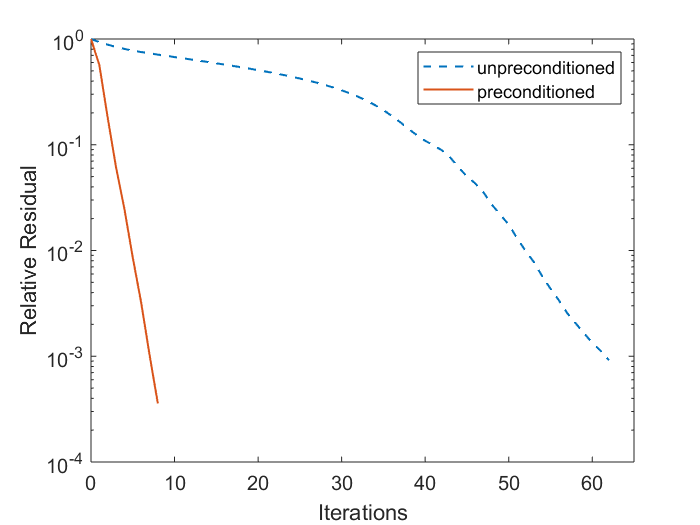
\includegraphics[height=6cm]{3_7_1.png}
    \caption{relative residual of PGMRES and GMRES.}
  \end{figure}
\end{exm}
%%% Local Variables:
%%% mode: latex
%%% TeX-master: "GMRES_MathDocument"
%%% End:
